\paragraph{}Esta es la página principal o de inicio de la aplicación web $\mu$Search. A esta página de inicio, el usuario o cliente habitual será siempre redirigido cuando pulse en cualquiera de los dos logotipos de la cabecera de la página.

\paragraph{}Se le muestra al usuario un mensaje de bienvenida y una breve descripción de en que consiste la página web $\mu$Search, de la empresa creadora y de que se ofrece a través del catálogo electronico.

\begin{figure}[h!]
	\centering
	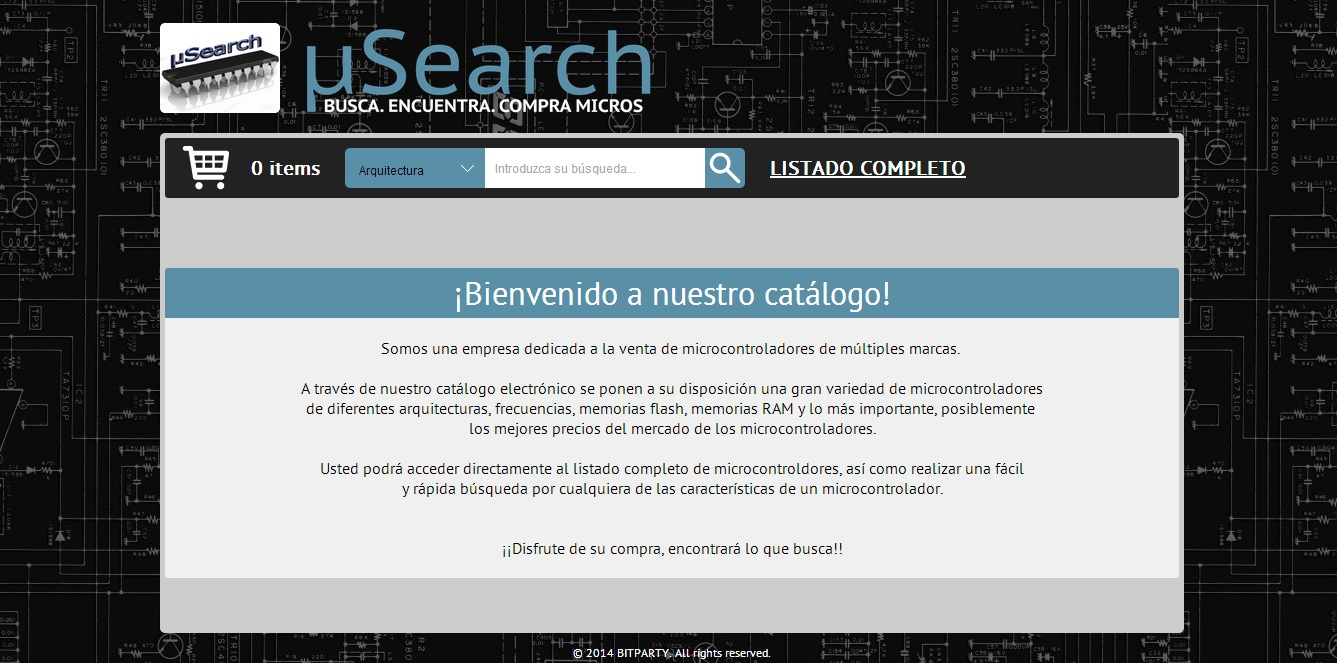
\includegraphics[width=0.85\textwidth]{img/principal_user}
	\caption{Página principal de usuario.}
	\label{fig:principal_usuario}
\end{figure}

Desde esta página, a través de los iconos situados en la cabecera debajo de los logotipos de la web, el usuario puede acceder a:
\begin{itemize}
	\item\textbf{Carrito de la compra:} Pulsando sobre este botón el usuario será redirigido a la página del carrito de la compra.
	
	\item \textbf{Búsqueda:} Desde esta sección de la cabecera, el usuario puede realizar búsquedas sobre el catálogo de microcontroladores en base a cualquiera de las diferentes características de un microcontrolador (Arquitectura, Frecuencia, Flash, RAM). Simplemente se debe seleccionar una de las características de la lista despegable, introducir el texto a buscar y pulsar sobre el icono de búsqueda.
	El usuario será redirigido a una página donde se le mostrará el resultado de la búsqueda en forma de lista de microcontroladores.
	
	\item \textbf{Listado Completo:} Pulsando sobre este botón/icono el sistema redirige al usuario a la página en la que se listan todos los elementos disponibles en el catálogo de microcontroladores.
	
\end{itemize}